\chapterimage{./Images/head2.jpg} % Chapter heading image
\chapter{Complex Numbers}
\section{Introduction}
\begin{definition}
    [Complex Numbers]
    $z$ is a complex number iff $z = a + bi$ where $a, b \in \mathbb{R}$ and $i^2 = -1$. \\
    The set of complex numbers is denoted by $\mathbb{C}$.
\end{definition}

\begin{definition}
    [Real and Imaginary Parts]
    If $z = a + bi$, then $\Re(z) = a \in \mathbb{R}$ and $\Im(z) = b \in \mathbb{R}$. where $\Re(z)$ is the real part of $z$ and $\Im(z)$ is the imaginary part of $z$.
\end{definition}

\begin{definition}
    [Modulus]
    If $z = a + bi$, then $|z| = \sqrt{a^2 + b^2}$. $|z|$ is the modulus of $z$.
\end{definition}

\begin{definition}
    [Conjugate]
    If $z = a + bi$, then $\overline{z} = a - bi$. $\overline{z}$ is the conjugate of $z$.
\end{definition}
\section{Operations}
\begin{definition}
    [Addition and Subtraction]
    If $z_1 = a_1 + b_1i$ and $z_2 = a_2 + b_2i$, then $z_1 + z_2 = (a_1 + a_2) + (b_1 + b_2)i$. \\
    Similarly $z_1 - z_2 = (a_1 - a_2) + (b_1 - b_2)i$.
\end{definition}

\begin{definition}
    [Multiplication]
    If $z_1 = a_1 + b_1i$ and $z_2 = a_2 + b_2i$, then $z_1 \cdot z_2 = (a_1a_2 - b_1b_2) + (a_1b_2 + a_2b_1)i$. \\
    \textit{    Note that $|z_1 \cdot z_2| = |z_1| \cdot |z_2|$.}
\end{definition}

\begin{definition}
    [Inversion]
    If $z = a + bi$, then $z^{-1} = \frac{\overline{z}}{|z|^2}= \frac{a}{a^2 + b^2} - \frac{b}{a^2 + b^2}i$.
\end{definition}
\begin{proof}
    Let's multiply by 1 in the form of the conjugate of $z$:
    \begin{align*}
        \frac{1}{z} = \frac{1}{z}\times \frac{\overline{z}}{\overline{z}} = \frac{\overline{z}}{z\overline{z}} = \frac{a - bi}{(a + bi)(a - bi)} = \frac{a - bi}{a^2 + b^2} = \frac{a}{a^2 + b^2} - \frac{b}{a^2 + b^2}i
    \end{align*}
\end{proof}

\begin{definition}
    [Division]
    For $z, w \in \mathbb{C}$, $\frac{w}{z} = w \cdot z^{-1} = \frac{w\overline{z}}{|z|^2}$.
\end{definition}
\begin{table}[htbp]
    \centering
    \caption{Properties of the Complex Conjugate}
    \begin{tabular}{|c|c|}
        \hline
        \textbf{Property}        & \textbf{Description}                                                              \\
        \hline
        Conjugate of the Sum     & $\overline{z_1 + z_2} = \overline{z_1} + \overline{z_2}$                          \\
        \hline
        Conjugate Modulus        & $ z \cdot \overline{z}= |z|^2$                                                    \\
        \hline
        Conjugate of a Conjugate & $\overline{\overline{z}} = z$                                                     \\
        \hline
        Product of Conjugates    & $\overline{z_1 \cdot z_2} = \overline{z_1} \cdot \overline{z_2}$                  \\
        \hline
        Conjugate of a Quotient  & $\overline{\left(\frac{z_1}{z_2}\right)} = \frac{\overline{z_1}}{\overline{z_2}}$ \\
        \hline
        Real Part Conjugate      & $Re(z) = \frac{z + \overline{z}}{2}$                                              \\
        \hline
        Imaginary Part Conjugate & $Im(z) = \frac{z - \overline{z}}{2i}$                                             \\
        \hline
        Real Number Check        & $z = \overline{z} \iff z \in \mathbb{R}$                                          \\
        \hline
        Imaginary Number Check   & $z = -\overline{z} \iff z \in \mathbb{I}$                                         \\
        \hline
        Function Linearity       & If $\alpha = f(z)$ then $\overline{\alpha} = \overline{f(z)} = f(\overline{z})$   \\
        \hline
    \end{tabular}
\end{table}

\begin{table}[htbp]
    \centering
    \caption{Properties of the Modulus in Complex Numbers}
    \begin{tabular}{|c|c|}
        \hline
        \textbf{Property}         & \textbf{Description}                                                           \\
        \hline
        Positivity                & $|z| \geq 0$, with equality if and only if $z = 0$                             \\
        \hline
        Triangle Inequality       & $||z_1| - |z_2|| \leq |z_1 \pm z_2| \leq |z_1| + |z_2|$                        \\
        \hline
        Multiplicative Property   & $|z_1 \cdot z_2| = |z_1| \cdot |z_2|$                                          \\
        \hline
        Division Property         & $\left|\frac{z_1}{z_2}\right| = \frac{|z_1|}{|z_2|}$, for $z_2 \neq 0$         \\
        \hline
        Conjugate                 & $|z| = |\overline{z}|$                                                         \\
        \hline
        Component Property        & $-|z| \leq Re(z) \leq |z|$                                                     \\ & $-|z| \leq Im(z) \leq |z|$ \\
        \hline
        Cauchy-Schwarz Inequality & $|z_1w_1 + \cdots + z_nw_n|^2 \leq \sum_{j=1}^{n}|z_j|^2\sum_{j=1}^{n}|w_j|^2$ \\
        \hline
    \end{tabular}
\end{table}

\begin{proof}
    Proof of the Multiplicative Property of the Modulus:
    \begin{align*}
        |z_1 \cdot z_2|^2 & = (z_1 \cdot z_2) \cdot (\overline{z_1} \cdot \overline{z_2}) \\
                          & = z_1 \cdot \overline{z_1} \cdot z_2 \cdot \overline{z_2}     \\
                          & = |z_1|^2 \cdot |z_2|^2
    \end{align*}
\end{proof}
\section{Polar Representation}
A complex number are vectors in $\mathbb{R}^2$, as such, they can be represented by a magnitude and a direction. \\

\begin{definition}[Polar Form]
    \begin{align}
         & z = r(\cos(\theta) + i\sin(\theta)) \label{polar} \\
         & : r = |z| \in \mathbb{R}^+ \notag
        \label{polar form}
    \end{align}
\end{definition}

\begin{figure}[htbp]
    \centering
    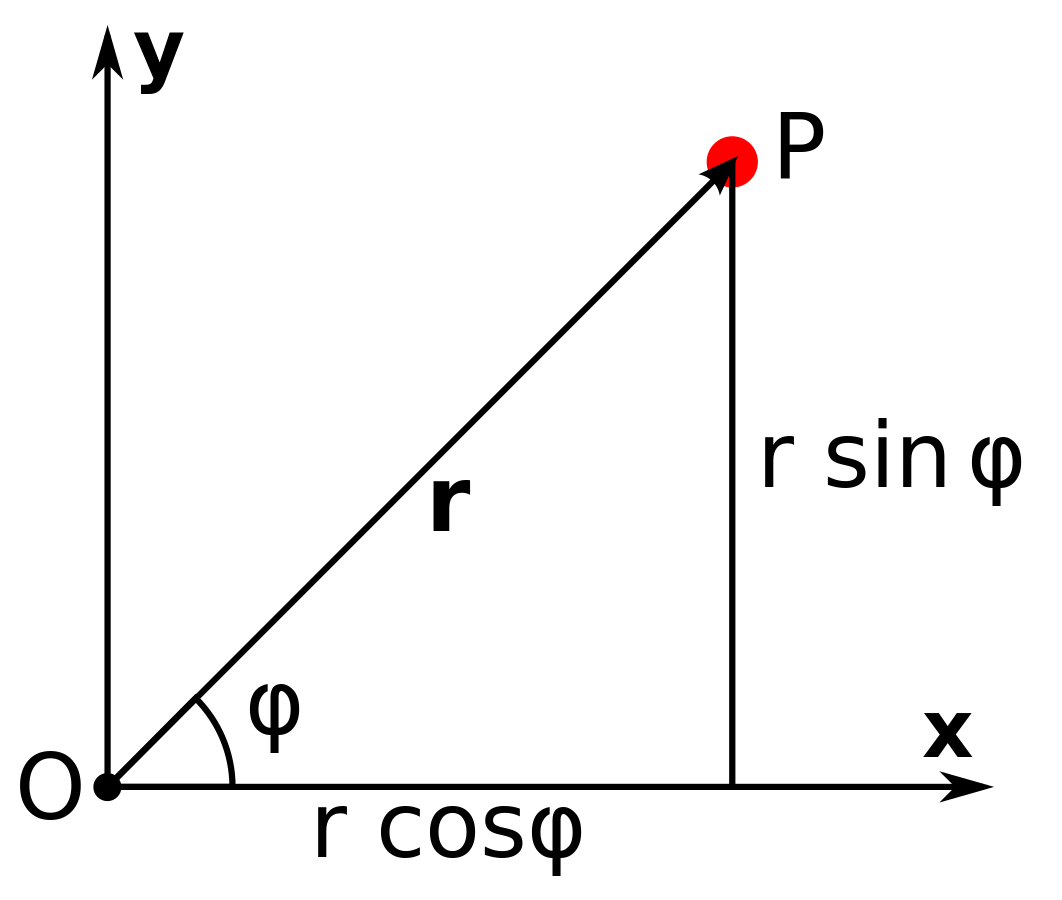
\includegraphics[scale = 0.2]{./LECTURE_1/Polar_coordinate_components.png}
    \caption{Polar Coordinate Components}
    \label{fig:polar}
\end{figure}

\begin{example}
    [Multiplying Complex Numbers in Polar Form]
    Let $z_1 = r_1(\cos(\theta_1) + i\sin(\theta_1))$ and $z_2 = r_2(\cos(\theta_2) + i\sin(\theta_2))$. Then:
    \begin{align}
        z_1 \cdot z_2 & = r_1r_2(\cos(\theta_1)\cos(\theta_2) - \sin(\theta_1)\sin(\theta_2) + i(\cos(\theta_1)\sin(\theta_2) + \sin(\theta_1)\cos(\theta_2))) \\
                      & = r_1r_2(\cos(\theta_1 + \theta_2) + i\sin(\theta_1 + \theta_2))
        \label{polar product}
    \end{align}
    Using the trig addition formula:
    \[\cos(\alpha + \beta) = \cos(\alpha)\cos(\beta) - \sin(\alpha)\sin(\beta)$ and $\sin(\alpha + \beta) = \cos(\alpha)\sin(\beta) + \sin(\alpha)\cos(\beta).\]
\end{example}

\begin{theorem}[De Moivre's Theorem]
    if $z = r(\cos(\theta) + i\sin(\theta))$
    \begin{align}
        z^n = r^n(\cos(\theta n) + i\sin(\theta n)) \label{Moivre}
    \end{align}
\end{theorem}

\begin{proof}
    \textit{The following proof will illustrative the steps to inductive reasoning}\\
    Case of $n = 1$: $z^n = r^n(\cos(\theta n) + i\sin(\theta n)) = z = r(\cos(\theta) + i\sin(\theta))$ \\
    This is true by definition. \\
    Assume that: \\
    $z^{n-1} = r^{n-1}(\cos(\theta (n-1)) + i\sin(\theta (n-1)))$ \\
    Then from Equation \eqref{polar product} we can verify: \\
    \begin{align}
        zz^{n-1} & = rr^{n-1}(\cos(\theta (n-1) + \theta) + i\sin(\theta (n-1) + \theta)) \notag \\
        z^{n}    & = r^{n}(\cos(\theta n) + i\sin(\theta n)) \notag
    \end{align}
\end{proof}

From Equation \eqref{polar}, we observe that $r$ is unique (because we constrained it to just positive values). $\theta$, however, is not unique.

\begin{definition}[Principle Orientation]
    We say $\theta$ is the principle orientation of $z$ if $\theta \in [-\pi, \pi)$ \\
    In this range, $\theta$ is unique.
\end{definition}

\begin{definition}
    [Vector Dot Product] The dot product of two vectors $a = (a_1, a_2)$ and $b = (b_1, b_2)$ is given by:
    \begin{align}
        a \cdot b  = \Re(a\overline{b})
        \label{dot product}
    \end{align}
\end{definition}

\begin{remark}
    [Complex Numbers to Solve Polynomial Equations]
    Over $\mathbb{C}$, every equation of the form $z^n = a$ has $n$ solutions.
\end{remark}
\begin{example}
    [Solving $z^n = -1$]
    Let $z = r(\cos(\theta) + i\sin(\theta))$. Then:
    \begin{align*}
        z^n               & = r^n(\cos(\theta n) + i\sin(\theta n)) = -1                                                               \\
        \implies r^n      & = 1 \text{ and } \cos(\theta n) + i\sin(\theta n) = -1                                                     \\
        \implies r        & = 1 \text{ and } \cos(\theta n) = -1 \text{ and } \sin(\theta n) = 0                                       \\
        \implies \theta n & = \pi + 2\pi k \text{ for } k \in \mathbb{Z}                                                               \\
        \implies \theta   & = \frac{\pi + 2\pi k}{n} \text{ for } k \in \mathbb{Z}                                                     \\
                          & \text{We can now find the principle solutions for } Z                                                      \\
                          & \therefore \theta_0 = \frac{\pi}{n}, \theta_1 = \frac{3\pi}{n}, \ldots, \theta_{n-1} = \frac{(2n-1)\pi}{n}
    \end{align*}
\end{example}
\begin{remark}
    Roots of Unity
    The solutions to $z^n = 1$ are called the $n$th roots of unity. Plotting these solutions splits the complex plane into $n$ equal parts.
    \begin{figure}
        \centering
        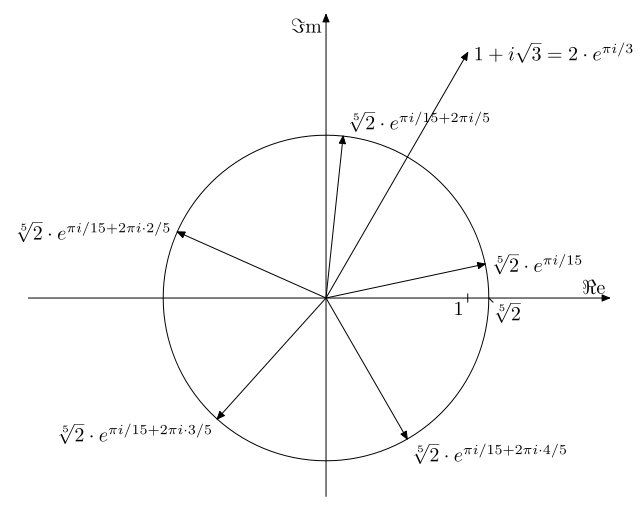
\includegraphics[scale = 0.2]{./LECTURE_1/Complex_fifth_roots.png}
        \caption{Complex Fifth Roots of Unity}
        \label{fig:roots}
    \end{figure}
\end{remark}
\section{Subsets of the Plane}
\begin{definition}
    [Open Disc]
    An open disc of radius $r$ centered at $z_0$ is the set of all $z$ such that $D = \{|z - z_0| < R\}$.
\end{definition}
\begin{definition}
    [Interior Point]
    A point $z_0$ is an interior point of a set $D \subset \mathbb{C}$ if there exists an open disc centered at $z_0$ that is contained in $D$.
\end{definition}

\begin{definition}
    [Open Set]
    A set $D \subset \mathbb{C}$ is open if every point in $D$ is an interior point.
\end{definition}

\begin{example}
    [Open Disc]
    Show that the disc $D = \{z \in \mathbb{C} : |z - z_0| < R\}$ is an open set.
    \begin{proof}
        Let $z_1 \in D$. Then $|z_1 - z_0| < R$. Let $r = R - |z_1 - z_0|$. Then $r > 0$. \\
        Let $z_2 \in D$ such that $|z_2 - z_1| < r$. Then:
        \begin{align*}
            |z_2 - z_0| & \leq |z_2 - z_1| + |z_1 - z_0| \\
                        & < r + R - r = R
        \end{align*}
        Therefore $z_2 \in D$ and $D$ is open.
    \end{proof}
\end{example}

\begin{definition}
    [Boundary ($\partial D$)]
    The boundary of a set $D$ is the set of all points $z$ such that every open disc centered at $z$ contains points in $D$ and points not in $D$. \\
    The boundary of $D$ is denoted by $\partial D$ and a boundary point $z$ is denoted by $z \in \partial D$.
\end{definition}

\begin{definition}
    [Closed Set]
    A set $D$ is closed if it contains all its boundary points.
\end{definition}
\begin{remark}
    A set can be both open and closed ($\mathbb{C}, \emptyset$), open and not closed, closed and not open, or neither open nor closed.
\end{remark}
\begin{theorem}
    [Properties of Open and Closed Sets]
    \begin{enumerate}
        \item $D$ is open iff $\mathbb{C} \setminus D$ is closed.
        \item $D$ is closed iff $\mathbb{C} \setminus D$ is open.
        \item $D$ is open if and only if it contains none of its boundary points.
    \end{enumerate}
\end{theorem}